\documentclass[aspectratio=169, 12pt]{beamer}

% ──────────────────────────────────────────────
% THEME & COLOR SETUP — Modern Minimal
% ──────────────────────────────────────────────
\usetheme{default}
\usecolortheme{default}
\usefonttheme{professionalfonts}

% Remove ALL navigation & footers
\setbeamertemplate{navigation symbols}{}
\setbeamertemplate{footline}{}
\setbeamertemplate{headline}{}

% ── Color Palette (Deep Navy + Electric Cyan accent) ──
\definecolor{bgDark}{HTML}{0D1117}
\definecolor{bgCard}{HTML}{161B22}
\definecolor{accentCyan}{HTML}{58A6FF}
\definecolor{accentPurple}{HTML}{BC8CFF}
\definecolor{accentGreen}{HTML}{3FB950}
\definecolor{accentOrange}{HTML}{F0883E}
\definecolor{accentRed}{HTML}{F85149}
\definecolor{textPrimary}{HTML}{E6EDF3}
\definecolor{textSecondary}{HTML}{8B949E}
\definecolor{borderGlow}{HTML}{30363D}

% Apply colors globally
\setbeamercolor{background canvas}{bg=bgDark}
\setbeamercolor{normal text}{fg=textPrimary}
\setbeamercolor{frametitle}{fg=textPrimary}
\setbeamercolor{title}{fg=white}
\setbeamercolor{subtitle}{fg=accentCyan}
\setbeamercolor{author}{fg=textSecondary}
\setbeamercolor{date}{fg=textSecondary}
\setbeamercolor{itemize item}{fg=accentCyan}
\setbeamercolor{itemize subitem}{fg=accentPurple}
\setbeamercolor{itemize subsubitem}{fg=accentGreen}
\setbeamercolor{block title}{fg=white, bg=bgCard}
\setbeamercolor{block body}{fg=textPrimary, bg=bgCard}

% Itemize markers
\setbeamertemplate{itemize item}{\small\raise1pt\hbox{\textcolor{accentCyan}{\textbullet}}}
\setbeamertemplate{itemize subitem}{\footnotesize\raise1pt\hbox{\textcolor{accentPurple}{--}}}

% Frame title template — thin accent bar, single-line
\setbeamertemplate{frametitle}{%
  \vspace{4pt}%
  \noindent\hspace{8pt}{\usebeamerfont{frametitle}\usebeamercolor[fg]{frametitle}\insertframetitle}%
  \vspace{2pt}%
  \par\noindent\hspace{8pt}{\color{accentCyan}\rule{0.97\textwidth}{0.8pt}}%
  \vspace{-2pt}%
}

% ── Typography ──
\usepackage[T1]{fontenc}
\usepackage{lmodern}
\setbeamerfont{title}{size=\LARGE, series=\bfseries}
\setbeamerfont{subtitle}{size=\normalsize}
\setbeamerfont{frametitle}{size=\normalsize, series=\bfseries}
\setbeamerfont{framesubtitle}{size=\small}
\setbeamerfont{author}{size=\small}
\setbeamerfont{date}{size=\footnotesize}

% ── Packages ──
\usepackage{graphicx}
\graphicspath{{../results/}{results/}}
\usepackage{tikz}
\usetikzlibrary{calc, positioning, shapes.geometric, arrows.meta, decorations.pathmorphing, backgrounds, fit}
\usepackage{booktabs}
\usepackage{xcolor}
\usepackage{ragged2e}
\usepackage{multicol}
\usepackage{textcomp}
\usepackage{amssymb}

% ──────────────────────────────────────────────
% CUSTOM COMMANDS
% ──────────────────────────────────────────────
\newcommand{\accentbox}[2]{%
  \begin{tikzpicture}
    \node[fill=bgCard, rounded corners=6pt, inner sep=10pt, 
          draw=borderGlow, line width=0.5pt, text width=0.9\textwidth, align=left] {%
      {\color{#1}\bfseries\large #2}%
    };
  \end{tikzpicture}%
}

\newcommand{\statbox}[3]{%
  \begin{tikzpicture}
    \node[fill=bgCard, rounded corners=6pt, inner sep=8pt, 
          draw=#1, line width=1pt, minimum width=2.8cm, align=center] {%
      {\color{#1}\fontsize{20}{24}\selectfont\bfseries #2}\\[2pt]%
      {\color{textSecondary}\scriptsize #3}%
    };
  \end{tikzpicture}%
}

% Icon replacements (simple text symbols)
\newcommand{\iconRobot}{\textcolor{accentCyan}{$\diamondsuit$}}
\newcommand{\iconCode}{\textcolor{accentOrange}{\texttt{\{.\}}}}
\newcommand{\iconTool}{\textcolor{accentGreen}{$\triangleright$}}
\newcommand{\iconLoop}{\textcolor{accentPurple}{$\circlearrowleft$}}
\newcommand{\iconQ}{\textcolor{accentCyan}{?}}
\newcommand{\iconCog}{\textcolor{accentGreen}{$\diamond$}}
\newcommand{\iconChart}{\textcolor{accentPurple}{$\square$}}
\newcommand{\iconChip}{\textcolor{accentCyan}{$\boxtimes$}}
\newcommand{\iconDB}{\textcolor{accentOrange}{$\boxplus$}}
\newcommand{\iconDisk}{\textcolor{accentPurple}{$\boxminus$}}
\newcommand{\iconWarn}{\textcolor{accentRed}{$\blacktriangle$}}
\newcommand{\iconX}{\textcolor{accentRed}{$\times$}}
\newcommand{\iconCheck}{\textcolor{accentGreen}{$\checkmark$}}
\newcommand{\iconBolt}{\textcolor{accentCyan}{$\ast$}}
\newcommand{\iconArrow}{\textcolor{accentCyan}{$\rightarrow$}}
\newcommand{\iconUp}{\textcolor{accentGreen}{$\uparrow$}}
\newcommand{\iconFire}{\textcolor{accentOrange}{$\star$}}
\newcommand{\iconGauge}{\textcolor{accentGreen}{$\bigstar$}}

% ──────────────────────────────────────────────
% DOCUMENT
% ──────────────────────────────────────────────
\begin{document}

% ═══════════════════════════════════════════════
% SLIDE 1: TITLE
% ═══════════════════════════════════════════════
{
\setbeamertemplate{background}{%
  \begin{tikzpicture}[remember picture, overlay]
    % Gradient mesh background
    \fill[bgDark] (current page.south west) rectangle (current page.north east);
    % Decorative glowing orbs
    \fill[accentCyan, opacity=0.08] (current page.north west) ++(4,-3) circle (5cm);
    \fill[accentPurple, opacity=0.06] (current page.south east) ++(-5,4) circle (6cm);
    \fill[accentGreen, opacity=0.04] (current page.center) ++(2,1) circle (3cm);
    % Grid lines
    \foreach \x in {0,0.5,...,16} {
      \draw[borderGlow, opacity=0.15, line width=0.2pt] (\x,0) -- (\x,9);
    }
    \foreach \y in {0,0.5,...,9} {
      \draw[borderGlow, opacity=0.15, line width=0.2pt] (0,\y) -- (16,\y);
    }
  \end{tikzpicture}%
}
\begin{frame}[plain]
  \vfill
  \begin{center}
    {\color{accentCyan}\fontsize{10}{12}\selectfont CMPT 450 \enspace$\cdot$\enspace SIMON FRASER UNIVERSITY}\\[18pt]
    {\color{white}\fontsize{26}{32}\selectfont\bfseries Beyond the GPU}\\[6pt]
    {\color{textSecondary}\fontsize{14}{18}\selectfont A Microarchitectural Analysis of}\\[2pt]
    {\color{accentCyan}\fontsize{14}{18}\selectfont LLM Tool-Calling Kernels}\\[28pt]
    {\color{textSecondary}\small Kunpeng Zhang \enspace\textcolor{borderGlow}{$|$}\enspace Fazal Rehman \enspace\textcolor{borderGlow}{$|$}\enspace TJ Grewal}\\[6pt]
    {\color{borderGlow}\footnotesize April 2026}
  \end{center}
  \vfill
\end{frame}
}

% ═══════════════════════════════════════════════
% SLIDE 2: THE PROBLEM — AGENTIC AI SHIFT
% ═══════════════════════════════════════════════
\begin{frame}{The Agentic AI Revolution}
  \begin{columns}[T]
    \begin{column}{0.52\textwidth}
      \vspace{6pt}
      {\color{textSecondary}\small LLMs have evolved from passive text generators to \textbf{\textcolor{accentCyan}{autonomous agents}} that:}
      \vspace{8pt}
      \begin{itemize}
        \item Invoke external APIs and tools
        \item Execute multi-step \textbf{ReAct} loops
        \item Parse structured JSON outputs
        \item Maintain growing context windows
      \end{itemize}
      \vspace{12pt}
      {\color{accentOrange}\bfseries The Problem:}\\[4pt]
      {\color{textSecondary}\small While the GPU has been relentlessly optimized, the \textbf{\textcolor{accentRed}{CPU orchestration overhead}} between reasoning steps remains largely \emph{uncharacterized}.}
    \end{column}
    \begin{column}{0.44\textwidth}
      \vspace{6pt}
      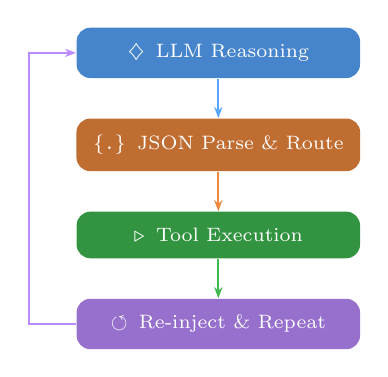
\begin{tikzpicture}[
        node distance=0.5cm,
        every node/.style={rounded corners=5pt, inner sep=6pt, font=\scriptsize, text=white, minimum width=3.6cm, align=center}
      ]
        \node[fill=accentCyan!80!black] (llm) {$\diamondsuit$\enspace LLM Reasoning};
        \node[fill=accentOrange!80!black, below=of llm] (parse) {\texttt{\{.\}}\enspace JSON Parse \& Route};
        \node[fill=accentGreen!80!black, below=of parse] (tool) {$\triangleright$\enspace Tool Execution};
        \node[fill=accentPurple!80!black, below=of tool] (inject) {$\circlearrowleft$\enspace Re-inject \& Repeat};
        
        \draw[-{Stealth[length=4pt]}, accentCyan, thick] (llm) -- (parse);
        \draw[-{Stealth[length=4pt]}, accentOrange, thick] (parse) -- (tool);
        \draw[-{Stealth[length=4pt]}, accentGreen, thick] (tool) -- (inject);
        \draw[-{Stealth[length=4pt]}, accentPurple, thick] (inject.west) -- ++(-0.6,0) |- (llm.west);
      \end{tikzpicture}
    \end{column}
  \end{columns}
\end{frame}

% ═══════════════════════════════════════════════
% SLIDE 3: RESEARCH QUESTION & CONTRIBUTIONS
% ═══════════════════════════════════════════════
\begin{frame}{Research Question}
  \vspace{4pt}
  \begin{center}
    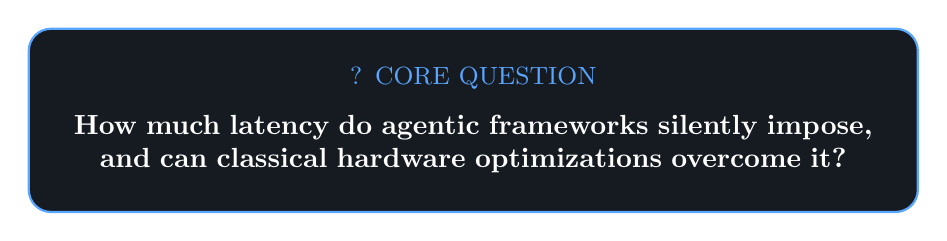
\begin{tikzpicture}
      \node[fill=bgCard, rounded corners=8pt, inner sep=14pt, 
            draw=accentCyan, line width=0.8pt, text width=0.85\textwidth, align=center] {%
        {\color{accentCyan}\small\iconQ\enspace CORE QUESTION}\\[6pt]
        {\color{white}\normalsize\bfseries How much latency do agentic frameworks silently impose,\\and can classical hardware optimizations overcome it?}
      };
    \end{tikzpicture}
  \end{center}
  \vspace{8pt}
  \begin{columns}[T]
    \begin{column}{0.48\textwidth}
      {\color{accentGreen}\scriptsize\iconCog\enspace METHODOLOGY}\\[4pt]
      \begin{itemize}\itemsep3pt
        \item[\textcolor{accentCyan}{\small 1.}] Decoupled profiling harness isolating CPU from GPU
        \item[\textcolor{accentCyan}{\small 2.}] PAPI hardware telemetry: cycles, IPC, L3 misses, branch mispredictions
      \end{itemize}
    \end{column}
    \begin{column}{0.48\textwidth}
      {\color{accentPurple}\scriptsize\iconChart\enspace KEY FINDINGS}\\[4pt]
      \begin{itemize}\itemsep3pt
        \item[\textcolor{accentPurple}{\small 3.}] Quantify the ``Agentic Tax'' across compute, memory, I/O domains
        \item[\textcolor{accentPurple}{\small 4.}] Identify the ``Masking Effect'' --- kernel wins vanish at system level
      \end{itemize}
    \end{column}
  \end{columns}
\end{frame}

% ═══════════════════════════════════════════════
% SLIDE 4: SYSTEM ARCHITECTURE
% ═══════════════════════════════════════════════
\begin{frame}{System Architecture}
  \begin{columns}[T]
    \begin{column}{0.50\textwidth}
      \vspace{4pt}
      {\color{textSecondary}\small Three strictly isolated layers:}
      \vspace{6pt}
      
      {\color{accentCyan}\bfseries\small 1. Orchestrator} {\color{textSecondary}\scriptsize (Python/FastAPI)}\\[2pt]
      {\color{textSecondary}\scriptsize Prompt assembly, tokenization, JSON routing}
      \vspace{6pt}
      
      {\color{accentGreen}\bfseries\small 2. Execution Kernels} {\color{textSecondary}\scriptsize (C++)}\\[2pt]
      {\color{textSecondary}\scriptsize Native binaries with internal PAPI profiling}
      \vspace{6pt}
      
      {\color{accentOrange}\bfseries\small 3. Static Workloads}\\[2pt]
      {\color{textSecondary}\scriptsize Pre-generated payloads for deterministic runs}
      \vspace{8pt}
      
      {\color{accentPurple}\bfseries\small Hardware Telemetry via PAPI:}
      \begin{itemize}\itemsep1pt
        {\scriptsize
        \item Total Cycles \& Instructions $\rightarrow$ IPC
        \item Branch Mispredictions
        \item L3 Cache Misses}
      \end{itemize}
    \end{column}
    \begin{column}{0.46\textwidth}
      \vspace{4pt}
      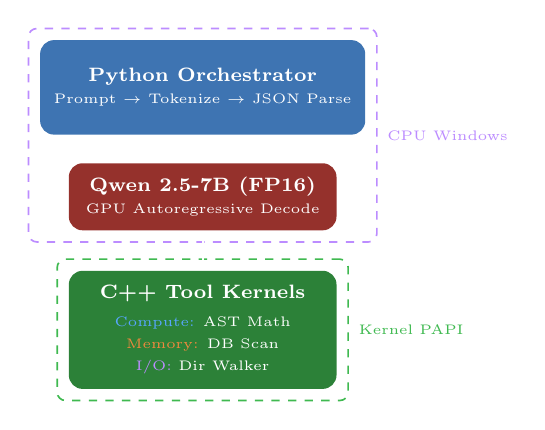
\begin{tikzpicture}[
        block/.style={rounded corners=5pt, inner sep=5pt, font=\scriptsize, text=white, minimum width=3.4cm, align=center, minimum height=0.8cm},
        node distance=0.35cm
      ]
        % Orchestrator block
        \node[block, fill=accentCyan!70!black, minimum height=1.2cm] (orch) {
          \textbf{Python Orchestrator}\\
          \tiny Prompt $\rightarrow$ Tokenize $\rightarrow$ JSON Parse
        };
        
        % GPU block
        \node[block, fill=accentRed!60!black, below=of orch] (gpu) {
          \textbf{Qwen 2.5-7B (FP16)}\\
          \tiny GPU Autoregressive Decode
        };
        
        % Kernels
        \node[block, fill=accentGreen!70!black, below=0.5cm of gpu, minimum height=1.5cm] (kern) {
          \textbf{C++ Tool Kernels}\\[2pt]
          \tiny \textcolor{accentCyan}{Compute:} AST Math\\
          \tiny \textcolor{accentOrange}{Memory:} DB Scan\\
          \tiny \textcolor{accentPurple}{I/O:} Dir Walker
        };
        
        % PAPI overlay
        \node[draw=accentPurple, dashed, line width=0.6pt, rounded corners=3pt, 
              fit=(orch)(gpu), inner sep=4pt, label={[font=\tiny, text=accentPurple]right:CPU Windows}] {};
        \node[draw=accentGreen, dashed, line width=0.6pt, rounded corners=3pt, 
              fit=(kern), inner sep=4pt, label={[font=\tiny, text=accentGreen]right:Kernel PAPI}] {};
        
        \draw[-{Stealth[length=3pt]}, white, thick] (orch) -- (gpu);
        \draw[-{Stealth[length=3pt]}, white, thick] (gpu) -- (kern);
      \end{tikzpicture}
    \end{column}
  \end{columns}
\end{frame}

% ═══════════════════════════════════════════════
% SLIDE 5: TOOL KERNELS
% ═══════════════════════════════════════════════
\begin{frame}{Tool Kernels}
  \vspace{4pt}
  \begin{columns}[c]
    \begin{column}{0.32\textwidth}
      \begin{center}
        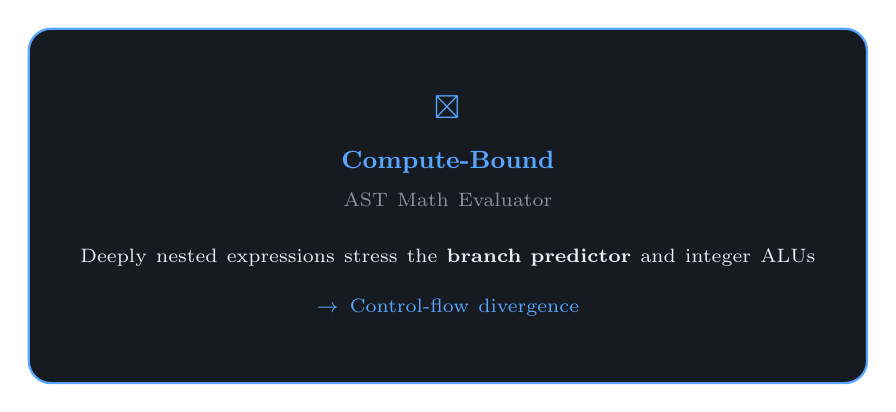
\begin{tikzpicture}
          \node[fill=bgCard, rounded corners=8pt, inner sep=10pt,
                draw=accentCyan, line width=0.8pt, text width=0.82\textwidth, align=center,
                minimum height=4.5cm] {%
            {\color{accentCyan}\large $\boxtimes$}\\[6pt]
            {\color{accentCyan}\bfseries\small Compute-Bound}\\[2pt]
            {\color{textSecondary}\scriptsize AST Math Evaluator}\\[8pt]
            {\color{textPrimary}\scriptsize Deeply nested expressions stress the \textbf{branch predictor} and integer ALUs}\\[6pt]
            {\color{accentCyan}\scriptsize$\rightarrow$\enspace Control-flow divergence}
          };
        \end{tikzpicture}
      \end{center}
    \end{column}
    \begin{column}{0.32\textwidth}
      \begin{center}
        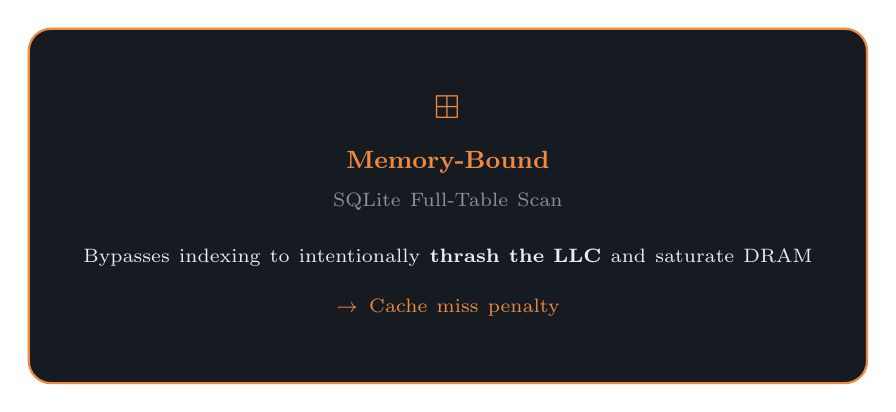
\begin{tikzpicture}
          \node[fill=bgCard, rounded corners=8pt, inner sep=10pt,
                draw=accentOrange, line width=0.8pt, text width=0.82\textwidth, align=center,
                minimum height=4.5cm] {%
            {\color{accentOrange}\large $\boxplus$}\\[6pt]
            {\color{accentOrange}\bfseries\small Memory-Bound}\\[2pt]
            {\color{textSecondary}\scriptsize SQLite Full-Table Scan}\\[8pt]
            {\color{textPrimary}\scriptsize Bypasses indexing to intentionally \textbf{thrash the LLC} and saturate DRAM}\\[6pt]
            {\color{accentOrange}\scriptsize$\rightarrow$\enspace Cache miss penalty}
          };
        \end{tikzpicture}
      \end{center}
    \end{column}
    \begin{column}{0.32\textwidth}
      \begin{center}
        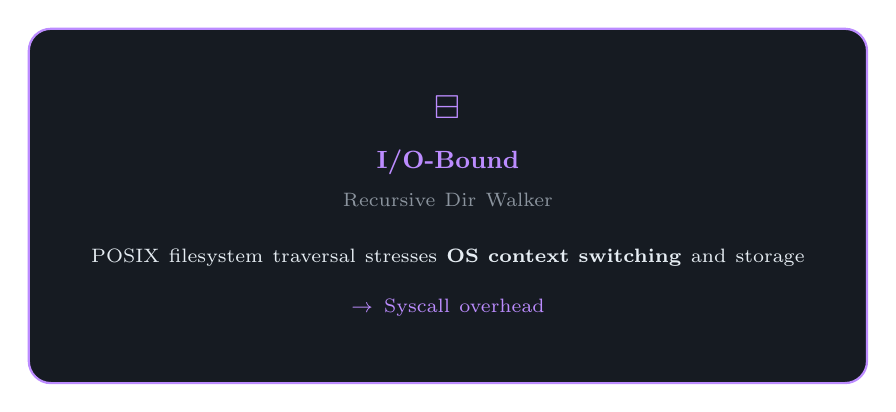
\begin{tikzpicture}
          \node[fill=bgCard, rounded corners=8pt, inner sep=10pt,
                draw=accentPurple, line width=0.8pt, text width=0.82\textwidth, align=center,
                minimum height=4.5cm] {%
            {\color{accentPurple}\large $\boxminus$}\\[6pt]
            {\color{accentPurple}\bfseries\small I/O-Bound}\\[2pt]
            {\color{textSecondary}\scriptsize Recursive Dir Walker}\\[8pt]
            {\color{textPrimary}\scriptsize POSIX filesystem traversal stresses \textbf{OS context switching} and storage}\\[6pt]
            {\color{accentPurple}\scriptsize$\rightarrow$\enspace Syscall overhead}
          };
        \end{tikzpicture}
      \end{center}
    \end{column}
  \end{columns}
\end{frame}

% ═══════════════════════════════════════════════
% SLIDE 6: THE AGENTIC TAX — KEY RESULT
% ═══════════════════════════════════════════════
{
\setbeamertemplate{background}{%
  \begin{tikzpicture}[remember picture, overlay]
    \fill[bgDark] (current page.south west) rectangle (current page.north east);
    \fill[accentRed, opacity=0.04] (current page.north east) ++(-6,-2) circle (7cm);
  \end{tikzpicture}%
}
\begin{frame}{Result 1: The Agentic Tax}
  \vspace{-2pt}
  \begin{center}
    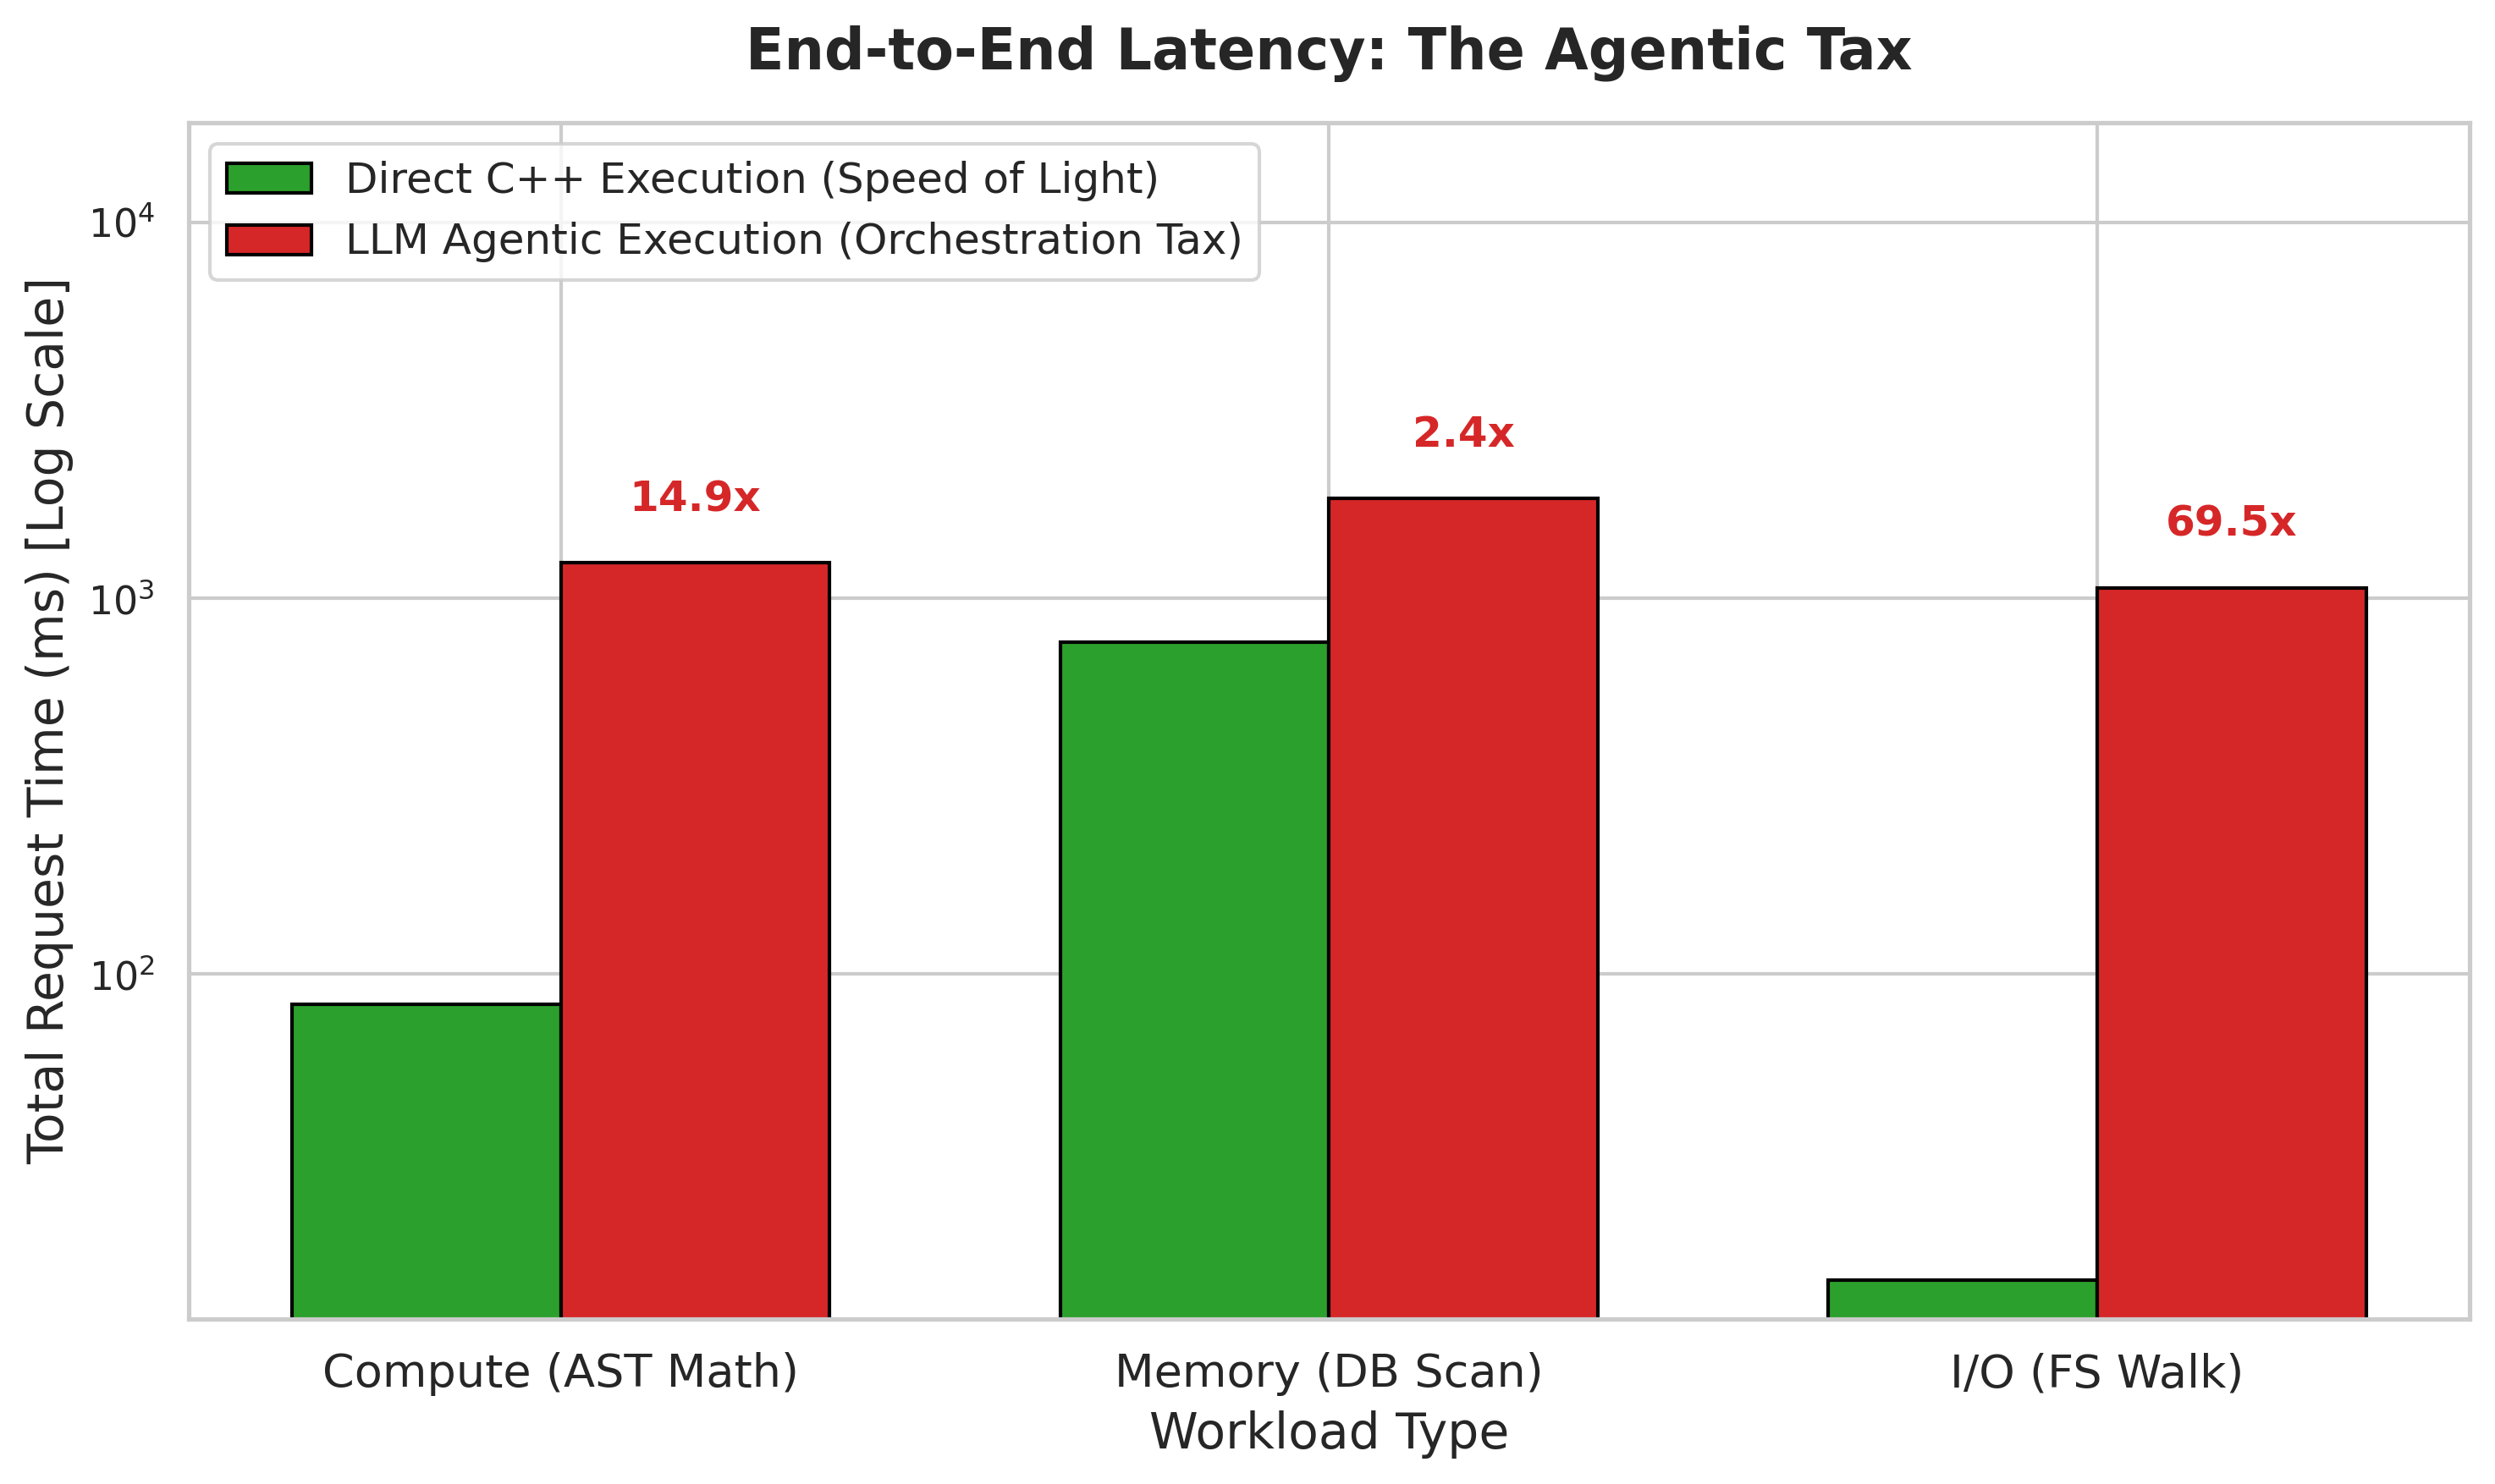
\includegraphics[width=0.72\textwidth, height=0.55\textheight, keepaspectratio]{ExpA_Agentic_Tax.png}
  \end{center}
  \vspace{-4pt}
  \begin{columns}[c]
    \begin{column}{0.32\textwidth}
      \centering\statbox{accentPurple}{69.5$\times$}{I/O Slowdown}
    \end{column}
    \begin{column}{0.32\textwidth}
      \centering\statbox{accentOrange}{14.9$\times$}{Compute Slowdown}
    \end{column}
    \begin{column}{0.32\textwidth}
      \centering\statbox{accentGreen}{2.4$\times$}{Memory Slowdown}
    \end{column}
  \end{columns}
\end{frame}
}

% ═══════════════════════════════════════════════
% SLIDE 7: INTERPRETING THE AGENTIC TAX
% ═══════════════════════════════════════════════
\begin{frame}{Interpreting the Agentic Tax}
  \vspace{6pt}
  \begin{center}
    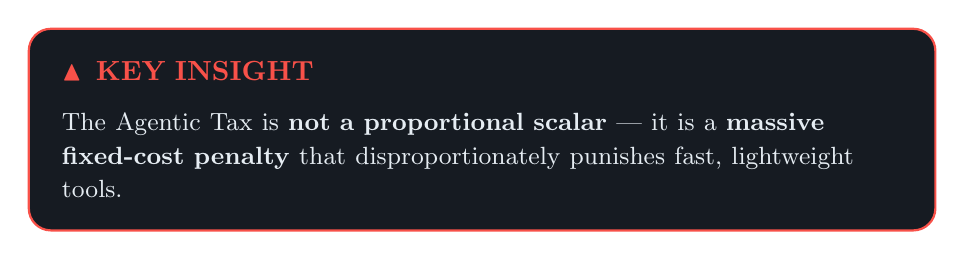
\begin{tikzpicture}
      \node[fill=bgCard, rounded corners=8pt, inner sep=12pt,
            draw=accentRed, line width=0.8pt, text width=0.88\textwidth, align=left] {%
        {\color{accentRed}\iconWarn\enspace\bfseries KEY INSIGHT}\\[6pt]
        {\color{textPrimary}\small The Agentic Tax is \textbf{not a proportional scalar} --- it is a \textbf{massive fixed-cost penalty} that disproportionately punishes fast, lightweight tools.}
      };
    \end{tikzpicture}
  \end{center}
  \vspace{6pt}
  \begin{columns}[T]
    \begin{column}{0.48\textwidth}
      {\color{accentPurple}\bfseries\small I/O Kernel (69.5$\times$)}\\[4pt]
      {\color{textSecondary}\scriptsize Native execution: $\sim$15ms\\
      GPU generation + Python serialization dwarf the actual filesystem walk}
      \vspace{8pt}
      
      {\color{accentOrange}\bfseries\small Compute Kernel (14.9$\times$)}\\[4pt]
      {\color{textSecondary}\scriptsize Fixed orchestration cost still dominates over the AST math evaluation time}
    \end{column}
    \begin{column}{0.48\textwidth}
      {\color{accentGreen}\bfseries\small Memory Kernel (2.4$\times$)}\\[4pt]
      {\color{textSecondary}\scriptsize Full-table scan requires $>$2.5 billion cycles ($\sim$764ms natively), so orchestration is a smaller fraction}
      \vspace{8pt}
      
      {\color{accentCyan}\bfseries\small Amdahl's Law at Work}\\[4pt]
      {\color{textSecondary}\scriptsize The heavier the native workload, the less proportional impact the fixed overhead has}
    \end{column}
  \end{columns}
\end{frame}

% ═══════════════════════════════════════════════
% SLIDE 8: MULTI-STEP ANALYSIS
% ═══════════════════════════════════════════════
\begin{frame}{Result 2: Multi-Step Workflow Analysis}
  \vspace{-2pt}
  \begin{center}
    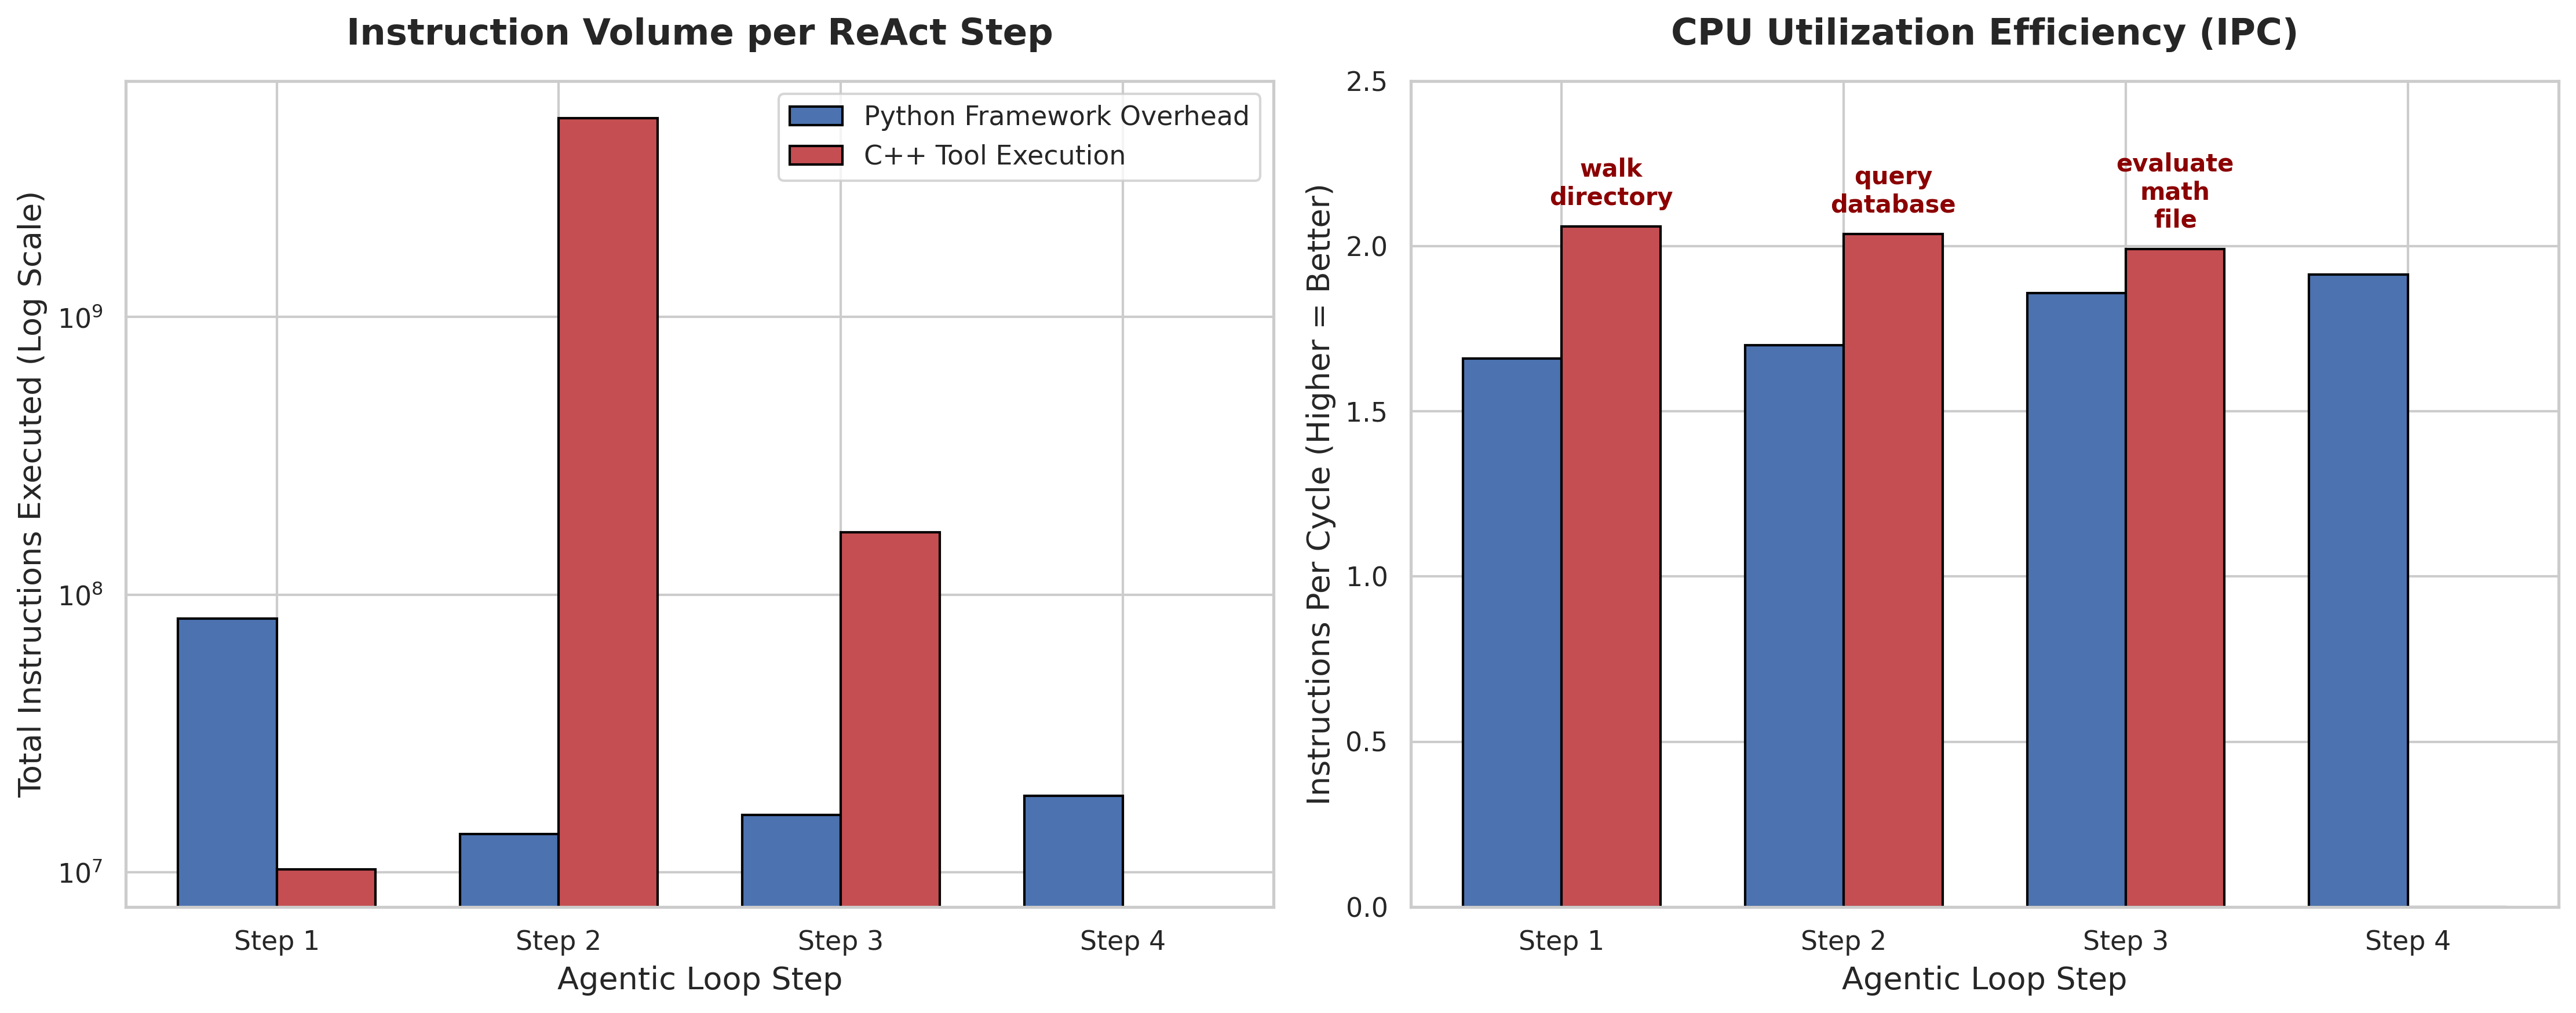
\includegraphics[width=0.82\textwidth, height=0.65\textheight, keepaspectratio]{ExpB_Multistep_Analysis.png}
  \end{center}
  \vspace{-4pt}
  {\color{textSecondary}\scriptsize\centering Left: Instruction volume (log scale). Right: IPC efficiency gap between framework and native tools.\par}
\end{frame}

% ═══════════════════════════════════════════════
% SLIDE 9: MULTI-STEP INSIGHTS
% ═══════════════════════════════════════════════
\begin{frame}{Multi-Step Insights}
  \vspace{6pt}
  \begin{columns}[T]
    \begin{column}{0.48\textwidth}
      {\color{accentCyan}\bfseries\small Framework Overhead}\\[6pt]
      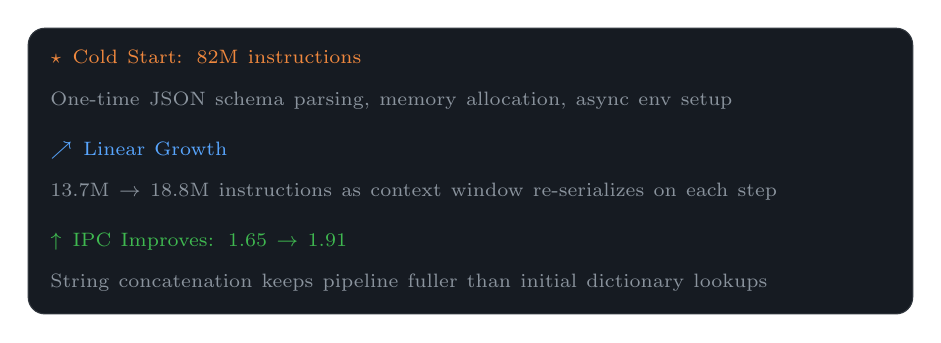
\begin{tikzpicture}
        \node[fill=bgCard, rounded corners=6pt, inner sep=8pt,
              draw=borderGlow, line width=0.4pt, text width=0.88\textwidth, align=left] {%
          {\color{accentOrange}\scriptsize\iconFire\enspace Cold Start: 82M instructions}\\[3pt]
          {\color{textSecondary}\scriptsize One-time JSON schema parsing, memory allocation, async env setup}\\[6pt]
          {\color{accentCyan}\scriptsize$\nearrow$\enspace Linear Growth}\\[3pt]
          {\color{textSecondary}\scriptsize 13.7M $\rightarrow$ 18.8M instructions as context window re-serializes on each step}\\[6pt]
          {\color{accentGreen}\scriptsize\iconUp\enspace IPC Improves: 1.65 $\rightarrow$ 1.91}\\[3pt]
          {\color{textSecondary}\scriptsize String concatenation keeps pipeline fuller than initial dictionary lookups}
        };
      \end{tikzpicture}
    \end{column}
    \begin{column}{0.48\textwidth}
      {\color{accentGreen}\bfseries\small C++ Tool Execution}\\[6pt]
      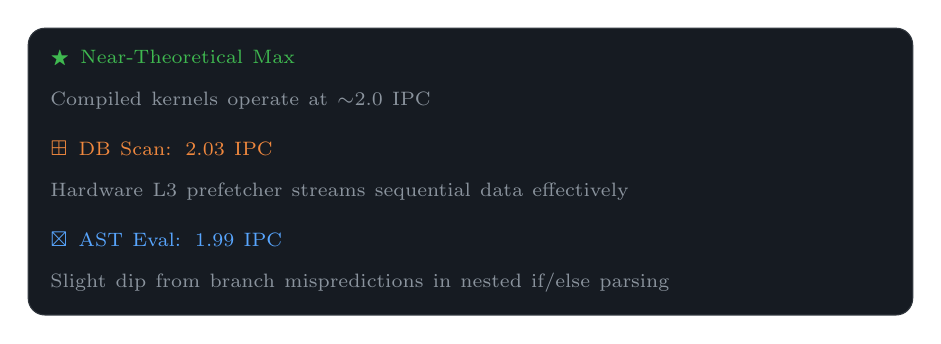
\begin{tikzpicture}
        \node[fill=bgCard, rounded corners=6pt, inner sep=8pt,
              draw=borderGlow, line width=0.4pt, text width=0.88\textwidth, align=left] {%
          {\color{accentGreen}\scriptsize\iconGauge\enspace Near-Theoretical Max}\\[3pt]
          {\color{textSecondary}\scriptsize Compiled kernels operate at $\sim$2.0 IPC}\\[6pt]
          {\color{accentOrange}\scriptsize$\boxplus$\enspace DB Scan: 2.03 IPC}\\[3pt]
          {\color{textSecondary}\scriptsize Hardware L3 prefetcher streams sequential data effectively}\\[6pt]
          {\color{accentCyan}\scriptsize$\boxtimes$\enspace AST Eval: 1.99 IPC}\\[3pt]
          {\color{textSecondary}\scriptsize Slight dip from branch mispredictions in nested if/else parsing}
        };
      \end{tikzpicture}
    \end{column}
  \end{columns}
\end{frame}

% ═══════════════════════════════════════════════
% SLIDE 10: OPTIMIZATION — VECTORIZATION WALL
% ═══════════════════════════════════════════════
\begin{frame}{Optimization 1: Vectorization Wall}
  \begin{columns}[T]
    \begin{column}{0.44\textwidth}
      \vspace{2pt}
      {\color{accentCyan}\bfseries\small Hypothesis}\\[3pt]
      {\color{textSecondary}\scriptsize AVX2 (256-bit SIMD) should accelerate numerical parsing throughput}
      \vspace{6pt}
      
      {\color{accentRed}\bfseries\small Reality}\\[3pt]
      {\color{textSecondary}\scriptsize Recursive control-flow divergence and pointer-chasing \textbf{completely neutralize} auto-vectorization}
      \vspace{6pt}
      
      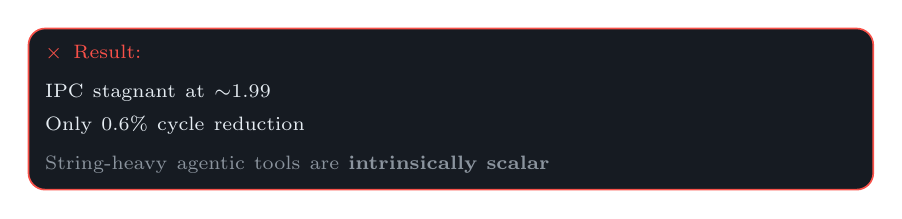
\begin{tikzpicture}
        \node[fill=bgCard, rounded corners=6pt, inner sep=6pt,
              draw=accentRed, line width=0.6pt, text width=0.85\textwidth, align=left] {%
          {\color{accentRed}\scriptsize\iconX\enspace Result:}\\[2pt]
          {\color{textPrimary}\scriptsize IPC stagnant at $\sim$1.99}\\
          {\color{textPrimary}\scriptsize Only 0.6\% cycle reduction}\\[2pt]
          {\color{textSecondary}\scriptsize String-heavy agentic tools are \textbf{intrinsically scalar}}
        };
      \end{tikzpicture}
    \end{column}
    \begin{column}{0.52\textwidth}
      \vspace{2pt}
      \begin{center}
        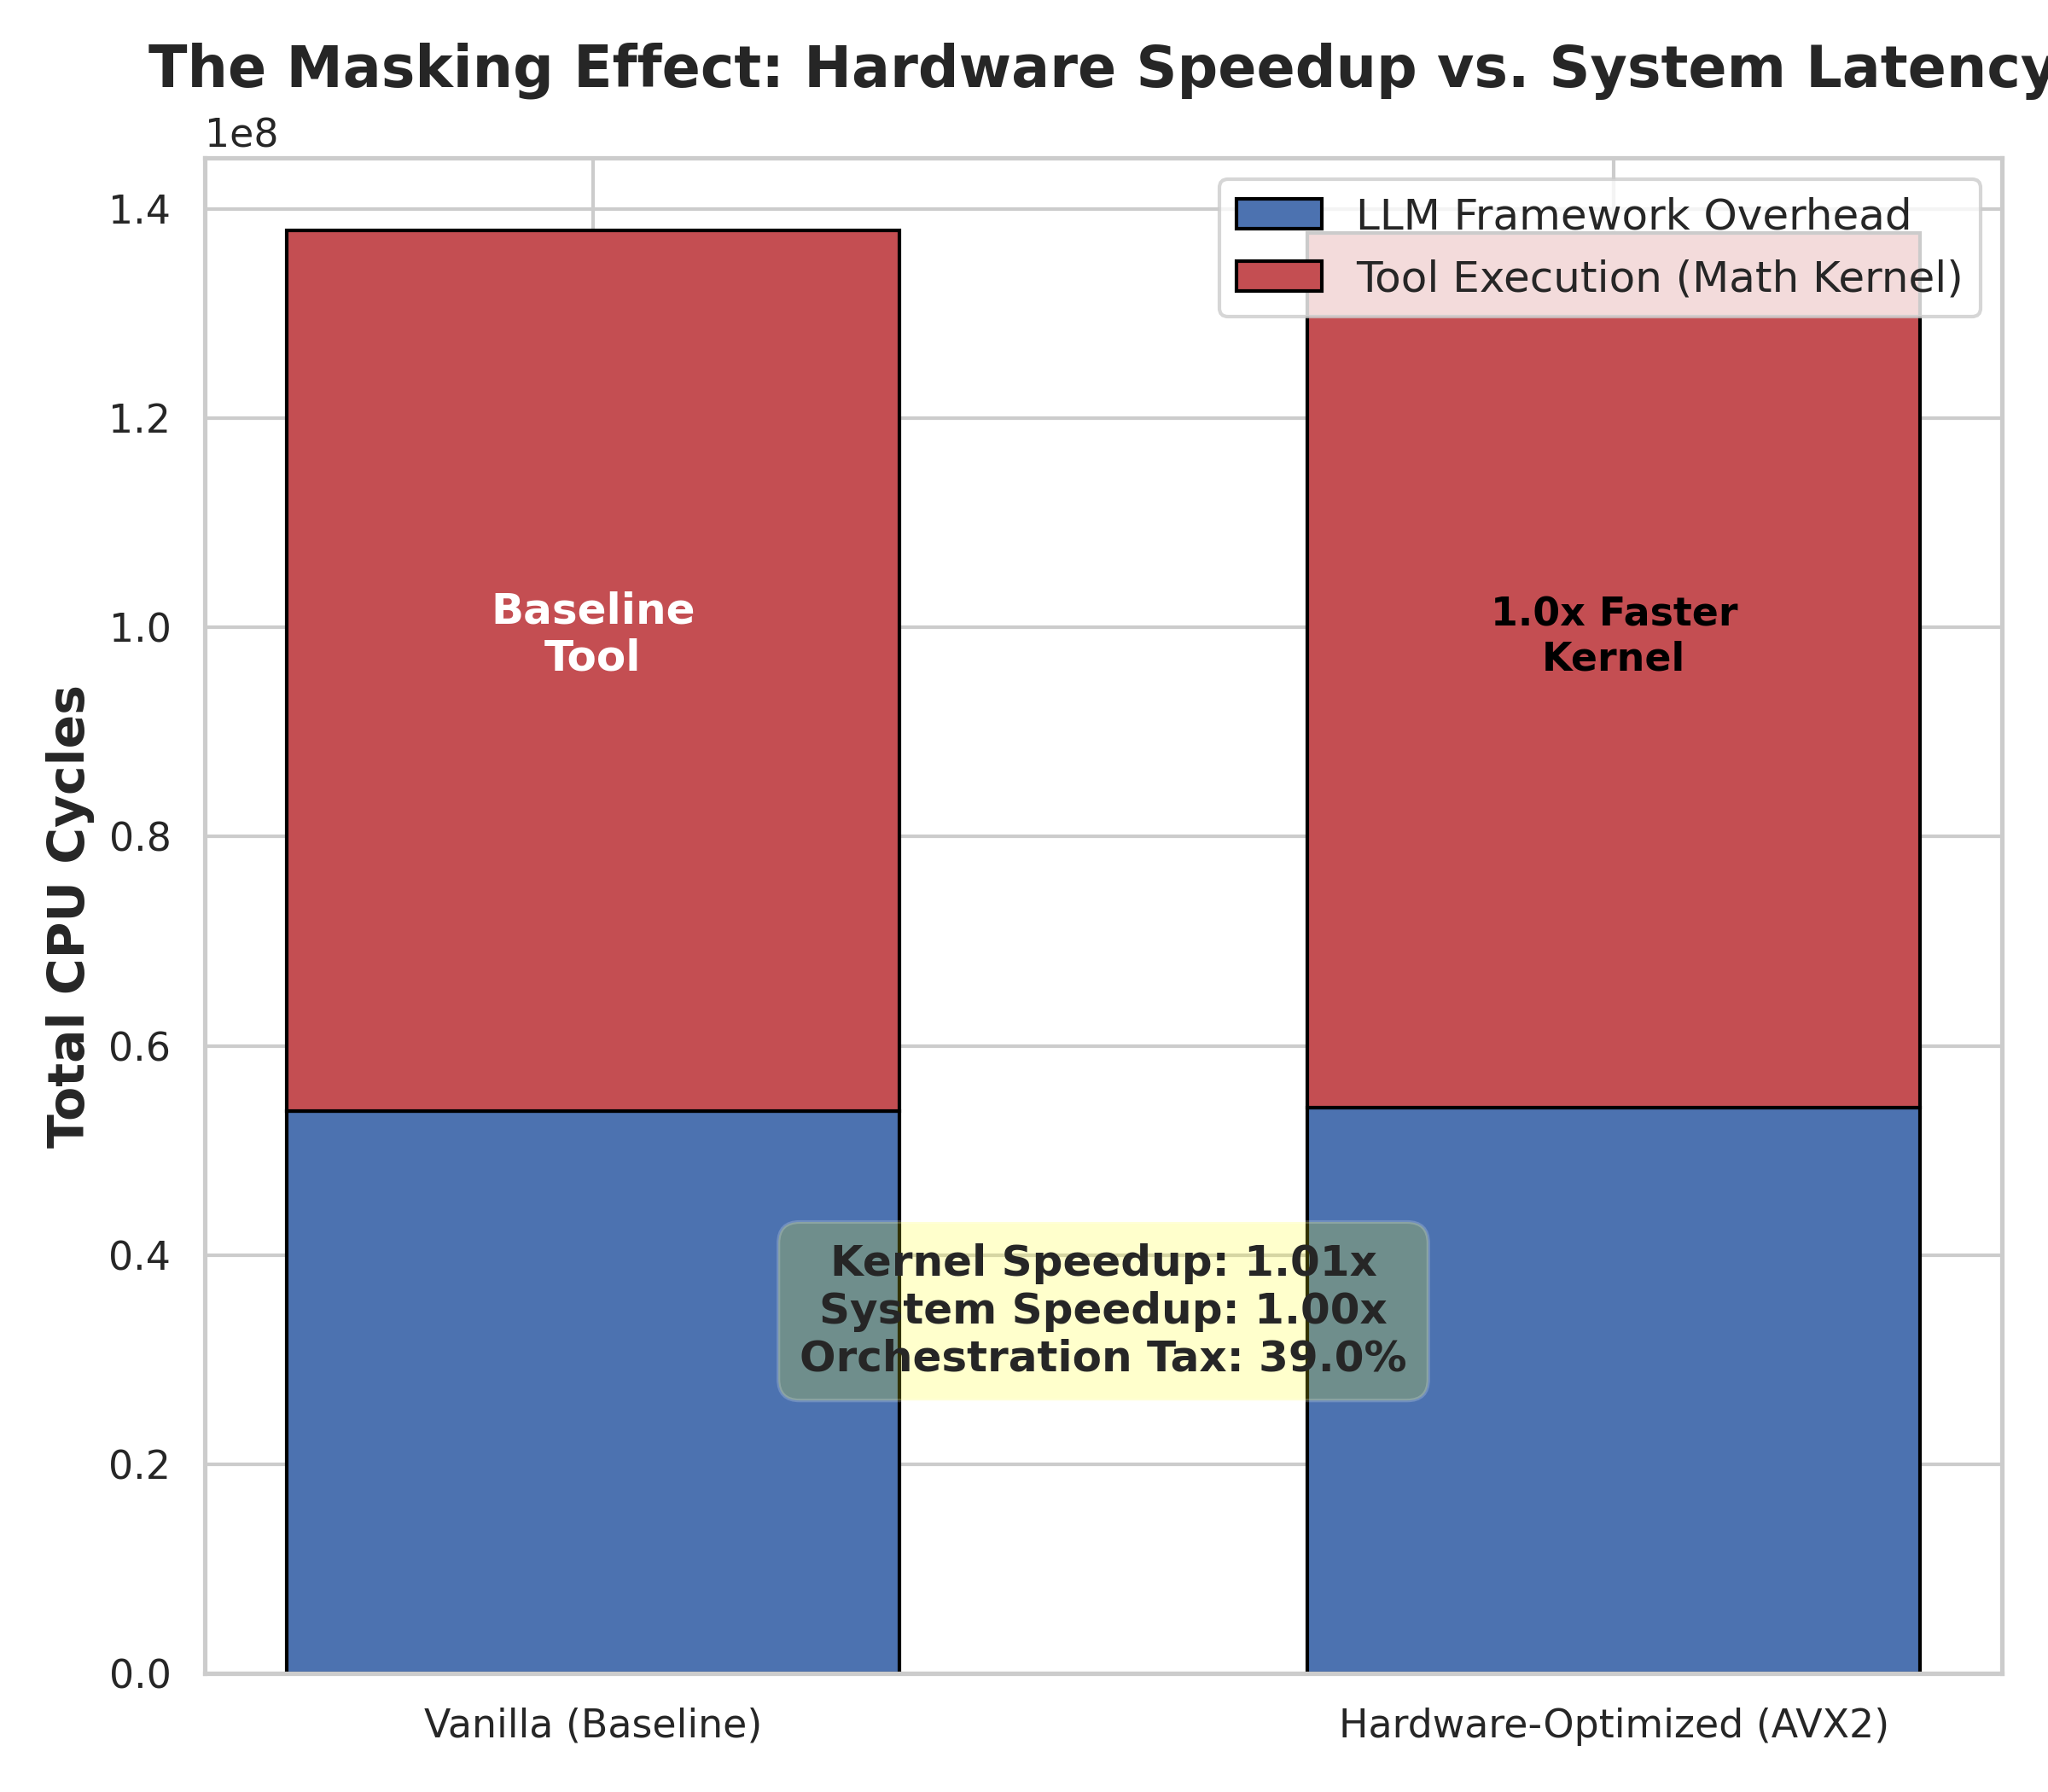
\includegraphics[width=0.95\textwidth, height=0.58\textheight, keepaspectratio]{Exp3_Masking_Effect.png}
      \end{center}
    \end{column}
  \end{columns}
\end{frame}

% ═══════════════════════════════════════════════
% SLIDE 11: OPTIMIZATION — SOFTWARE PREFETCHING
% ═══════════════════════════════════════════════
\begin{frame}{Optimization 2: Software Prefetching}
  \vspace{-2pt}
  \begin{center}
    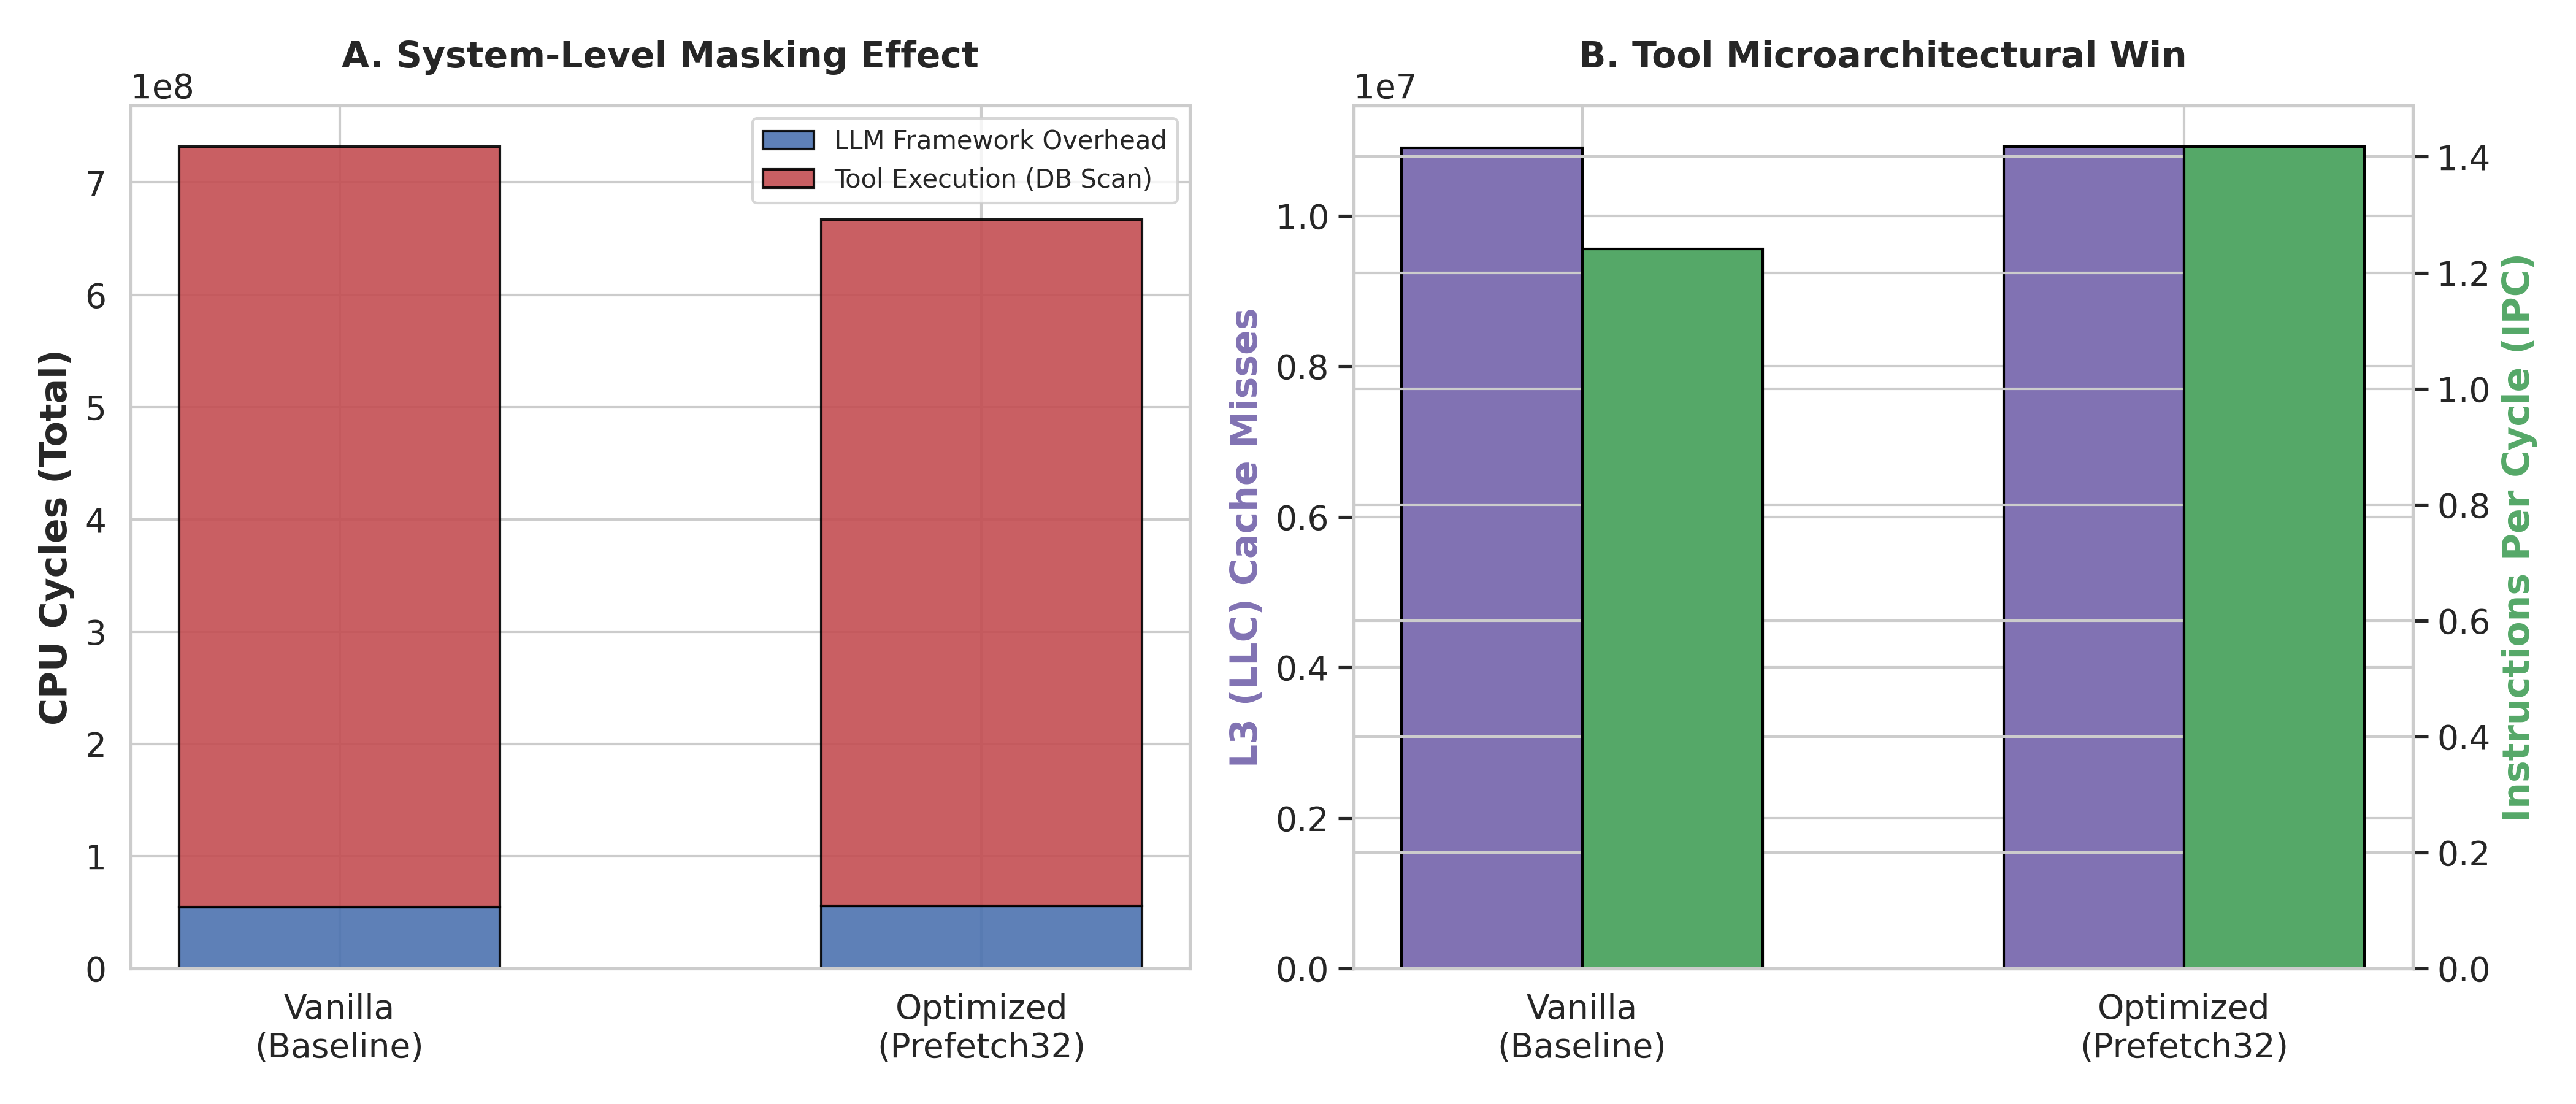
\includegraphics[width=0.72\textwidth, height=0.55\textheight, keepaspectratio]{Exp4_DB_Memory_Wall_Analysis.png}
  \end{center}
  \vspace{-4pt}
  \begin{columns}[c]
    \begin{column}{0.32\textwidth}
      \centering\statbox{accentGreen}{+14.2\%}{IPC Improvement}
    \end{column}
    \begin{column}{0.32\textwidth}
      \centering\statbox{accentCyan}{66M}{Cycles Saved}
    \end{column}
    \begin{column}{0.32\textwidth}
      \centering\statbox{accentOrange}{$\sim$50ms}{Wall-Clock Saving}
    \end{column}
  \end{columns}
\end{frame}

% ═══════════════════════════════════════════════
% SLIDE 12: THE MASKING EFFECT
% ═══════════════════════════════════════════════
{
\setbeamertemplate{background}{%
  \begin{tikzpicture}[remember picture, overlay]
    \fill[bgDark] (current page.south west) rectangle (current page.north east);
    \fill[accentRed, opacity=0.06] (current page.center) circle (6cm);
  \end{tikzpicture}%
}
\begin{frame}{Result 3: The Masking Effect}
  \vspace{-2pt}
  \begin{center}
    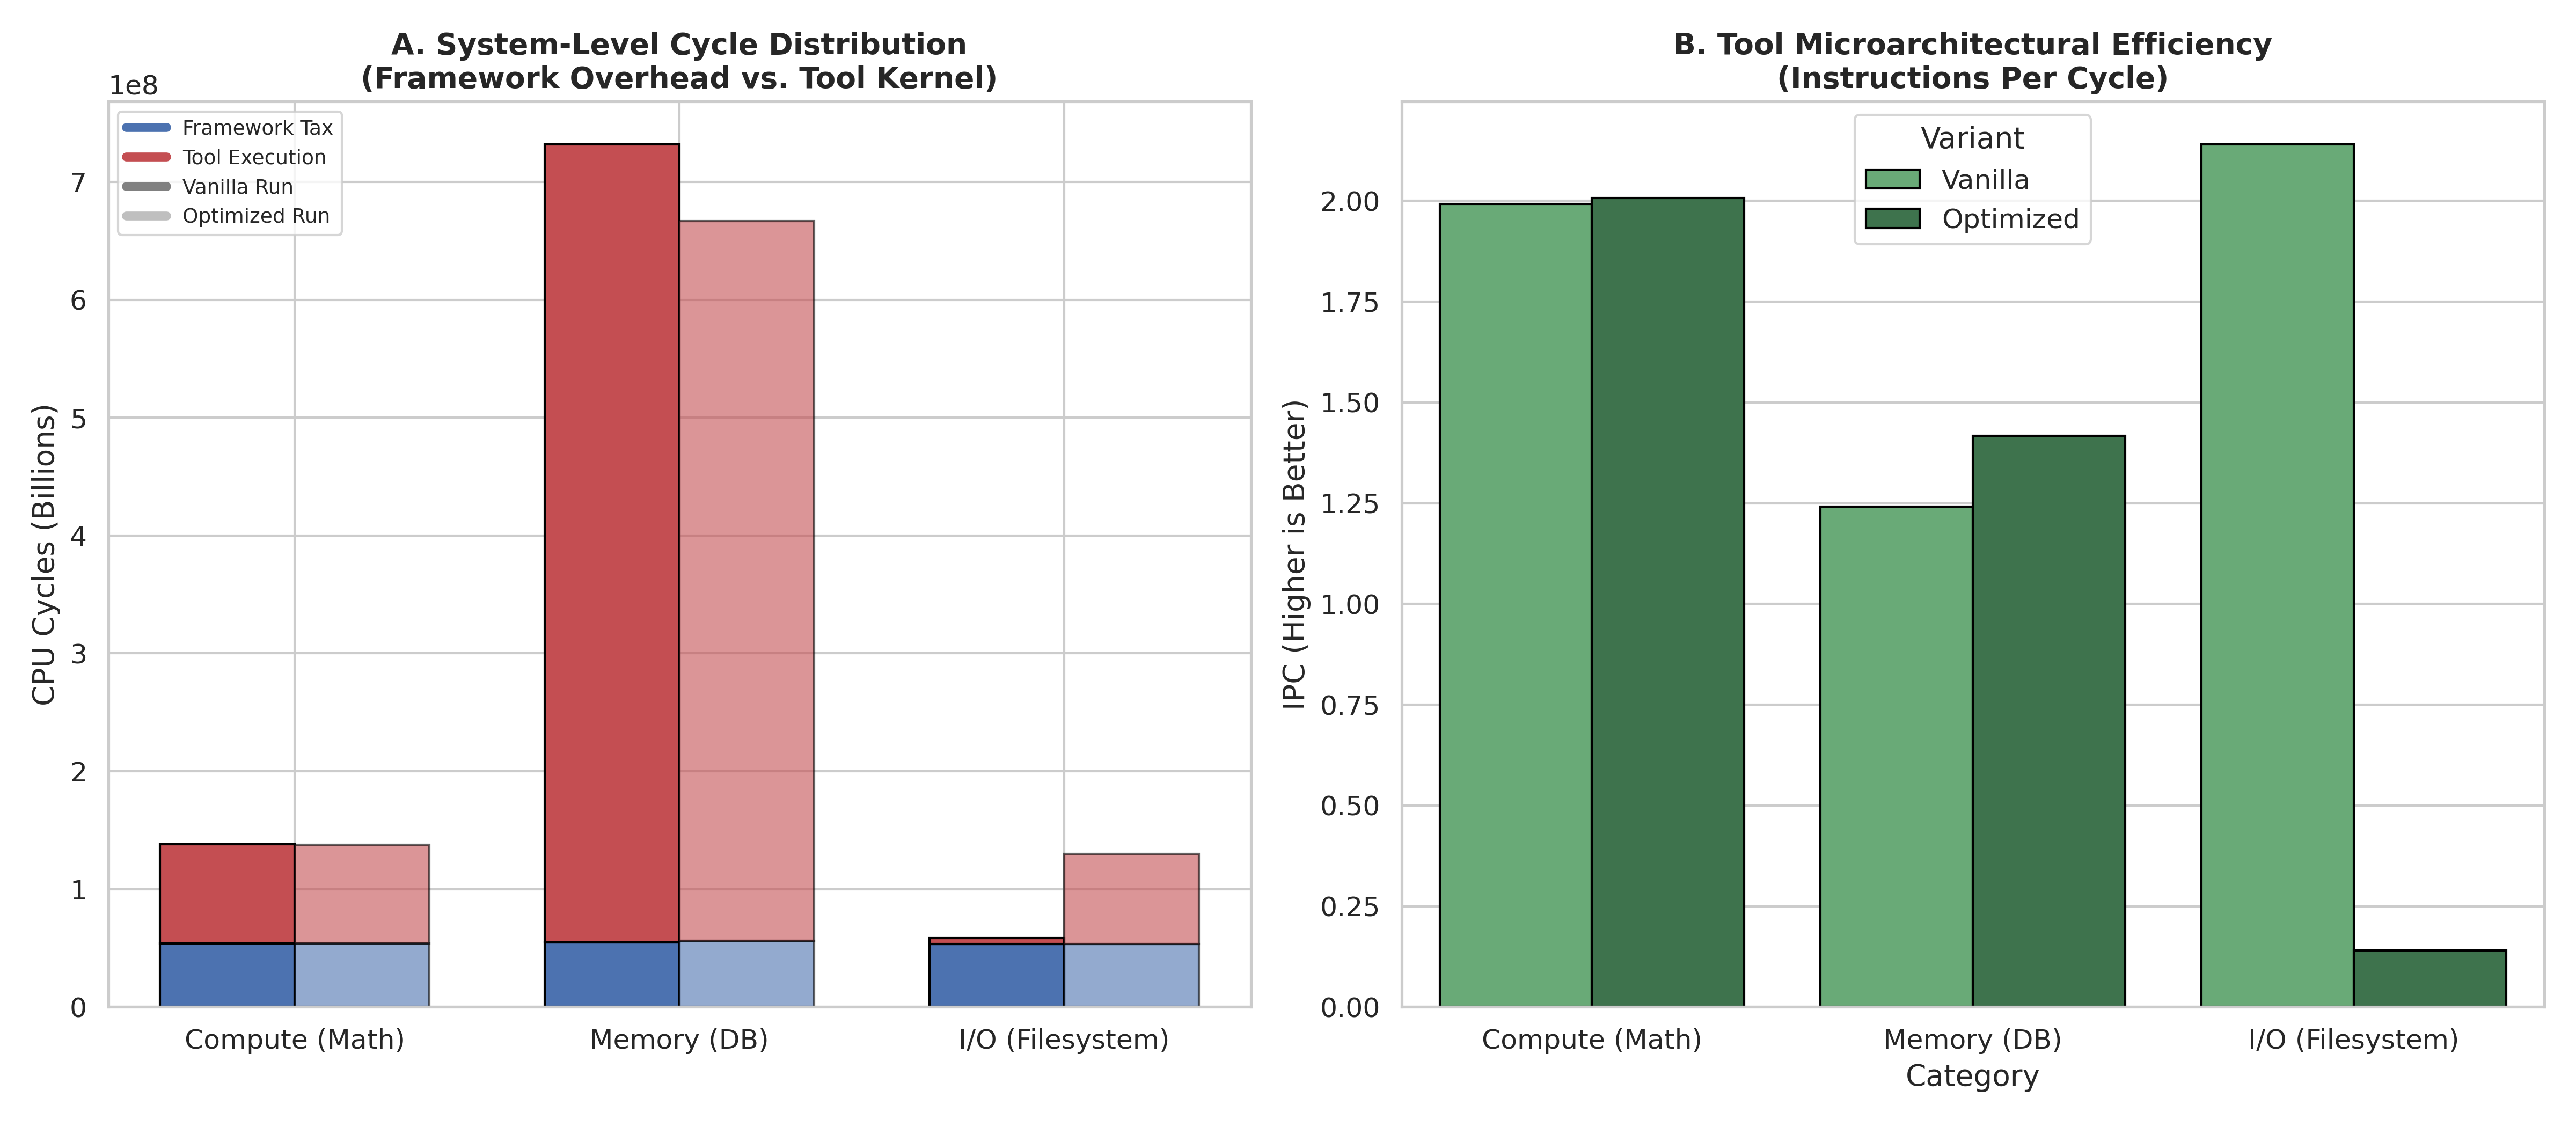
\includegraphics[width=0.72\textwidth, height=0.50\textheight, keepaspectratio]{Final_Research_Comparison.png}
  \end{center}
  \vspace{-4pt}
  \begin{center}
    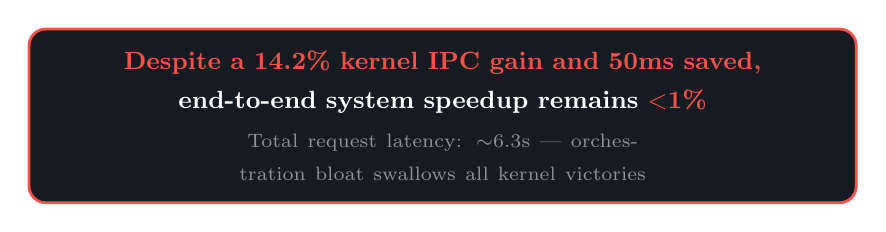
\begin{tikzpicture}
      \node[fill=bgCard, rounded corners=6pt, inner sep=8pt,
            draw=accentRed, line width=1pt, text width=0.82\textwidth, align=center] {%
        {\color{accentRed}\small\bfseries Despite a 14.2\% kernel IPC gain and 50ms saved,}\\[2pt]
        {\color{white}\small\bfseries end-to-end system speedup remains \textcolor{accentRed}{$<$1\%}}\\[2pt]
        {\color{textSecondary}\scriptsize Total request latency: $\sim$6.3s --- orchestration bloat swallows all kernel victories}
      };
    \end{tikzpicture}
  \end{center}
\end{frame}
}

% ═══════════════════════════════════════════════
% SLIDE 13: FUTURE WORK
% ═══════════════════════════════════════════════
\begin{frame}{Future Work}
  \vspace{4pt}
  \begin{columns}[T]
    \begin{column}{0.48\textwidth}
      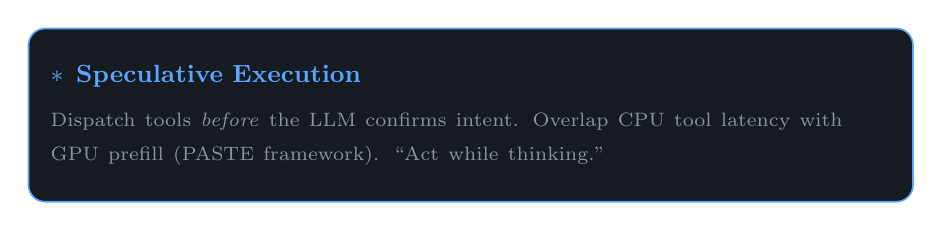
\begin{tikzpicture}
        \node[fill=bgCard, rounded corners=6pt, inner sep=8pt,
              draw=accentCyan, line width=0.6pt, text width=0.88\textwidth, align=left,
              minimum height=2.2cm] {%
          {\color{accentCyan}\small$\ast$\enspace\bfseries Speculative Execution}\\[4pt]
          {\color{textSecondary}\scriptsize Dispatch tools \emph{before} the LLM confirms intent. Overlap CPU tool latency with GPU prefill (PASTE framework). ``Act while thinking.''}
        };
      \end{tikzpicture}
      \vspace{6pt}
      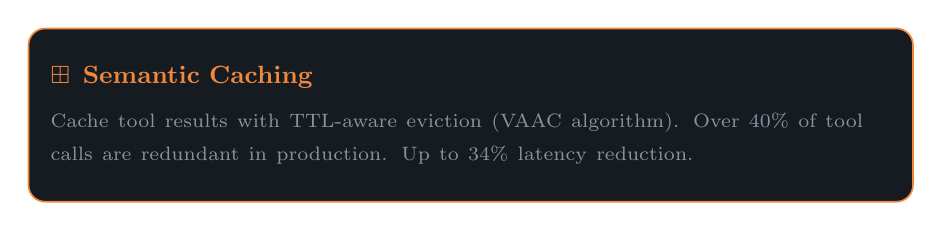
\begin{tikzpicture}
        \node[fill=bgCard, rounded corners=6pt, inner sep=8pt,
              draw=accentOrange, line width=0.6pt, text width=0.88\textwidth, align=left,
              minimum height=2.2cm] {%
          {\color{accentOrange}\small$\boxplus$\enspace\bfseries Semantic Caching}\\[4pt]
          {\color{textSecondary}\scriptsize Cache tool results with TTL-aware eviction (VAAC algorithm). Over 40\% of tool calls are redundant in production. Up to 34\% latency reduction.}
        };
      \end{tikzpicture}
    \end{column}
    \begin{column}{0.48\textwidth}
      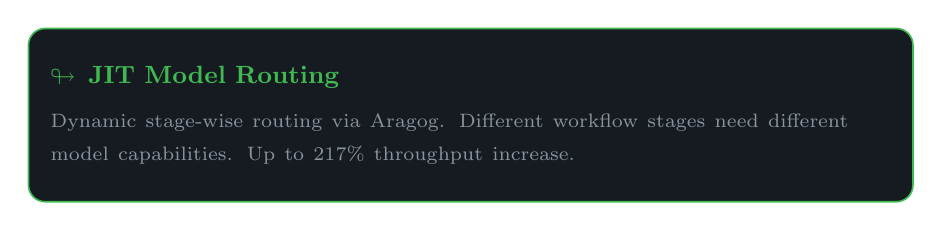
\begin{tikzpicture}
        \node[fill=bgCard, rounded corners=6pt, inner sep=8pt,
              draw=accentGreen, line width=0.6pt, text width=0.88\textwidth, align=left,
              minimum height=2.2cm] {%
          {\color{accentGreen}\small$\looparrowright$\enspace\bfseries JIT Model Routing}\\[4pt]
          {\color{textSecondary}\scriptsize Dynamic stage-wise routing via Aragog. Different workflow stages need different model capabilities. Up to 217\% throughput increase.}
        };
      \end{tikzpicture}
      \vspace{6pt}
      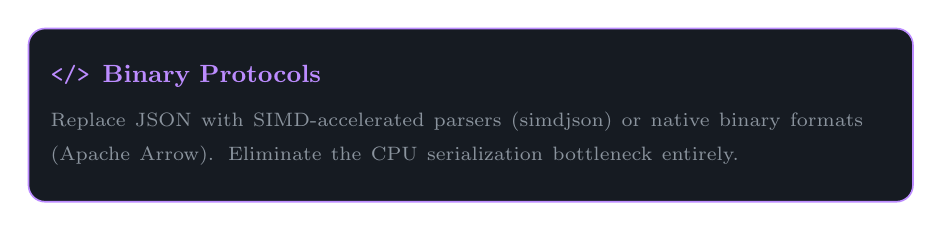
\begin{tikzpicture}
        \node[fill=bgCard, rounded corners=6pt, inner sep=8pt,
              draw=accentPurple, line width=0.6pt, text width=0.88\textwidth, align=left,
              minimum height=2.2cm] {%
          {\color{accentPurple}\small\texttt{</>}\enspace\bfseries Binary Protocols}\\[4pt]
          {\color{textSecondary}\scriptsize Replace JSON with SIMD-accelerated parsers (simdjson) or native binary formats (Apache Arrow). Eliminate the CPU serialization bottleneck entirely.}
        };
      \end{tikzpicture}
    \end{column}
  \end{columns}
\end{frame}

% ═══════════════════════════════════════════════
% SLIDE 14: CONCLUSION
% ═══════════════════════════════════════════════
{
\setbeamertemplate{background}{%
  \begin{tikzpicture}[remember picture, overlay]
    \fill[bgDark] (current page.south west) rectangle (current page.north east);
    \fill[accentCyan, opacity=0.06] (current page.south west) ++(5,3) circle (5cm);
    \fill[accentPurple, opacity=0.04] (current page.north east) ++(-4,-4) circle (4cm);
    % Grid
    \foreach \x in {0,0.5,...,16} {
      \draw[borderGlow, opacity=0.1, line width=0.2pt] (\x,0) -- (\x,9);
    }
    \foreach \y in {0,0.5,...,9} {
      \draw[borderGlow, opacity=0.1, line width=0.2pt] (0,\y) -- (16,\y);
    }
  \end{tikzpicture}%
}
\begin{frame}{Conclusion}
  \vspace{2pt}
  \begin{center}
    {\color{white}\large\bfseries The orchestration layer is the bottleneck.}\\[8pt]
    
    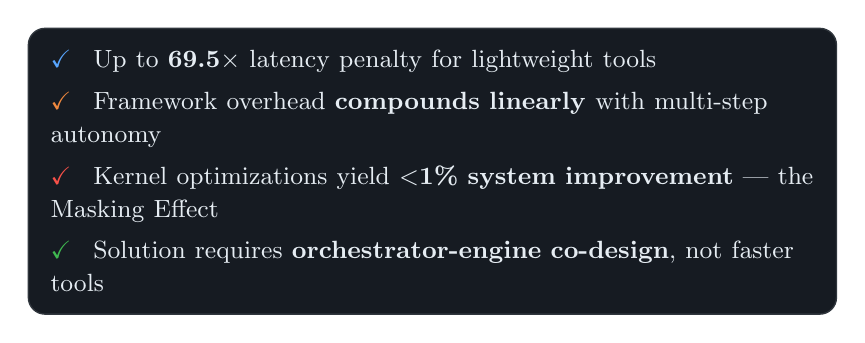
\begin{tikzpicture}
      \node[fill=bgCard, rounded corners=6pt, inner sep=8pt,
            draw=borderGlow, line width=0.5pt, text width=0.8\textwidth, align=left] {%
        {\color{accentCyan}\small$\checkmark$\enspace} {\color{textPrimary}\small Up to \textbf{69.5$\times$} latency penalty for lightweight tools}\\[3pt]
        {\color{accentOrange}\small$\checkmark$\enspace} {\color{textPrimary}\small Framework overhead \textbf{compounds linearly} with multi-step autonomy}\\[3pt]
        {\color{accentRed}\small$\checkmark$\enspace} {\color{textPrimary}\small Kernel optimizations yield \textbf{$<$1\% system improvement} --- the Masking Effect}\\[3pt]
        {\color{accentGreen}\small$\checkmark$\enspace} {\color{textPrimary}\small Solution requires \textbf{orchestrator-engine co-design}, not faster tools}
      };
    \end{tikzpicture}
    
    \vspace{8pt}
    {\color{textSecondary}\itshape\scriptsize ``Until the orchestration layer is treated as a high-performance\\networking data plane, the potential of hardware-accelerated\\agentic tools will remain hidden beneath the execution tax.''}
  \end{center}
\end{frame}
}

% ═══════════════════════════════════════════════
% SLIDE 15: THANK YOU
% ═══════════════════════════════════════════════
{
\setbeamertemplate{background}{%
  \begin{tikzpicture}[remember picture, overlay]
    \fill[bgDark] (current page.south west) rectangle (current page.north east);
    \fill[accentCyan, opacity=0.08] (current page.center) ++(0,1) circle (5cm);
    \fill[accentPurple, opacity=0.05] (current page.center) ++(3,-2) circle (4cm);
    \fill[accentGreen, opacity=0.04] (current page.center) ++(-4,-1) circle (3cm);
  \end{tikzpicture}%
}
\begin{frame}[plain]
  \vfill
  \begin{center}
    {\color{white}\fontsize{30}{36}\selectfont\bfseries Thank You}\\[10pt]
    {\color{accentCyan}\large Questions?}\\[24pt]
    {\color{textSecondary}\small Kunpeng Zhang \enspace$\cdot$\enspace Fazal Rehman \enspace$\cdot$\enspace TJ Grewal}\\[6pt]
    {\color{borderGlow}\footnotesize Simon Fraser University \enspace$\cdot$\enspace CMPT 450}
  \end{center}
  \vfill
\end{frame}
}

\end{document}
